\chapter{Álgebra vectorial}


\setcounter{section}{1}
\section{El espacio vectorial de las n-plas de números reales}

%--------------------definición 12.1.
\begin{tcolorbox}[colframe = white]
    \begin{def.} Dos vectores $A$ y $B$ de $V_n$ son iguales siempre que coinciden sus componentes. Esto es, si $A=(a_1,a_2,...,a_n)$ y $B=(b_1,b_2,...,b_3)$, la ecuación vectorial $A=B$ tiene exactamente el mismo significado que las $n$ ecuaciones escalares $$a_1=b_1, \qquad a_2=b_2, \qquad a_n=b_n$$
    La suma $A+B$ se define como el vector obtenido sumando los componentes correspondientes: $$A+B = (a_1+b_1,a_2+b_2,...,a_n+b_n)$$
    La $c$ es un escalar, definimos $cA$ o $Ac$ como el vector obtenido multiplicando cada componente de $A$ por $c$: $$cA=(ca_1,ca_2,...,ca_n)$$
    \end{def.}
\end{tcolorbox}

%--------------------teorema 12.1
\begin{teo}

\begin{enumerate}[\bfseries a.]
    \item La adición de vectores es conmutativa. $$A+B=B+A$$\\
	Demostración.-\; Sea $V_n$ el espacio vectorial n-plas y $A=(a_1,a_2,...,a_n)$ y $B=(b_1,b_2,...b_n)$, por lo tanto por definición de adición  y propiedad de números reales, tenemos $$A+B = (a_1+b_1,a_2+b_2,...,a_n+b_n) = (b_1+a_1,b_2+a_2,...,b_n+a_n) = B+A$$.\\

    \item y asociativa, $$A+(B+C) = (A+B)+C$$\\
	Demostración.-\; Sea $V_n$ el espacio vectorial n-plas y $A = (a_1,a_2,...,a_n)$, $B=(b_1,b_2,...,b_n)$ y $C=(c_1,c_2,...,c_n)$ entonces $$A+(B+C) = A + (b_1+c_1,b_2+c_2,...,b_n+c_n) = (a_1+(b_1+c_1),a_2+(b_2+c_2),...,a_1+(b_n+c_n)) = $$
	$$((a_1+b_1)+c_1,(a_2+b_2)+c_2,...,(a_n+b_n)+c_n) = (a_1+b_1,a_2+b_2,...,b_n+c_n)+C = (A+B)+C$$\\

    \item La multiplicación por escalares es asociativa $$c(dA)=(cd)A$$\\
	Demostración.-\; Sea $c,d \in \mathbb{R}$ y $A\in V_n$ entonces 
	\begin{center}
	    \begin{tabular}{rcl}
		$c(dA)$&$=$&$c(da_1,da_2,...,da_n)$\\
		&$=$&$((cd)a_1,(cd)a_2,...,(cd)a_3)$\\
		&$=$&$(cd)A$\\\\
	    \end{tabular}
	\end{center}

    \item y satisface las dos leyes distributivas $$c(A+B)=cA+cB,\quad y \quad (c+d)A=cA+dA$$\\
	Demostración.-\; Las demostraciones son fáciles de realizar siempre y cuando se tomen en cuenta Las definiciones de 12.1.\\\\

    \item El vector con todos los componentes $0$ se llama vector cero y se representa con $O$. Tiene la propiedad.\\\\
	Demostración.-\; Existencia. Sea $O = (o,o,...,o)$ de donde $A+O = (a_1,a_2,...,a_n)+(o,o,...,o) = (a_1+o,a_2+o,...,a_n+o) = (a_1,a_2,...,a_n) = A$.\\
	Unicidad. Supongamos que $O,O^{'} \in V_n; O\neq O$ tal que 
	$$\left\{ \begin{array}{ccc} A+O=A&tomando \; A=O^{'}:&O^{'}+O = O^{'}\\ A+O^{'} = A&tomando \; A=O:&O+O^{'}=O\\ \end{array} \right.$$
	Por lo tanto $O=O^{'}$.\\\\
    \item El vector $(-1)A$ que también se representa con $-A$ se llama el apuesto a $A$. También escribimos $A-B$ en lugar de $A+(-B)$ y lo llamamos diferencia de $A$ y $B$. La ecuación $(A+B)-B=A$. Demuestra que la sustracción es la operación inversa de la adición. Obsérvese que $0A=O$ y que $1A=A$.\\\\

\end{enumerate}
    
\end{teo}

\section{Interpretación geométrica para $n\leq 3$}

%--------------------definición 12.2
\begin{tcolorbox}[colframe = white]

    \begin{def.} Dos vectores $A$ y $B$ de $V_n$ tienen la misma dirección si $B=cA$ para un cierto escalar positivo $c$, y la dirección opuesta si $B=cA$ para un cierto $c$ negativo. Se llaman paralelos si $B=cA$ para un cierto $c$ no nulo.
    \end{def.}
\end{tcolorbox}

\section{Ejercicios}
\begin{enumerate}[\large\bfseries 1.]

%--------------------1.
\item Sean $A=(1,3,6)$, $B=(4,-3,3)$ y $C=(2,1,5)$ tres vectores de $V_3$. Determinar los componentes de cada uno de los vectores: 
\begin{enumerate}[\bfseries a)]

    %----------a)
    \item $A+B = (1,3,6) + (4,-3,3) = (1+4,3+(-3),6+3) = (5,0,9)$\\\\

    %----------b)
    \item $A-B = (1,3,6) - (4,-3,3) = (1-4,3-(-3),6-3) = (-3,6,3)$\\\\

    %----------c)
    \item $A+B-C = (1,3,6)+(4,-3,3)-(2,1,5) = (1+4-2,3-3-1,6+3-5) = (3,-1,4)$\\\\

    %----------d)
    \item $7A-2B-3C = 7(1,3,6)-2(4,-3,3)-3(2,1,5) = (7,21,42)-(8,-6,6)-(6,3,15) =$\\ $=(7-8-6,21-8-(-6)-3,42-6-15) = (-7,24,21)$\\\\

    %----------e)
    \item $2A+B-3C = 2(1,3,6) + (4,-3,3) 3(2,1,5) = (2+4-6,6-3-3,12+3-15) = (0,0,0)$\\\\

\end{enumerate}

%--------------------2.
\item Dibujar los vectores geométricos que unen el origen a los puntos $A=(2,1)$ y $B=(1,3).$ En la misma figura trazar el vector geométrico que une el origen al punto $C=A+t(B)$ para cada uno de los siguientes valores de $t$: $t=\frac{1}{2}$; $t=\frac{3}{4}$; $t=1;$ $t=2$; $t=-1$; $t=-2$.\\\\
    Respuesta.-\: 
    \begin{center}
	\begin{tabular}{clcl}
	    Si&$t=\frac{1}{3}$&$\Longrightarrow$&$C=(\frac{7}{3},2)$\\\\
	    Si & $t=\frac{1}{2}$ & $\Longrightarrow$ & $C=(\frac{5}{2},\frac{5}{2})$ \\\\
	    Si & $t=1$ & $\Longrightarrow$ & $C=(\frac{11}{4},\frac{13}{4})$ \\\\
	    Si & $t=2$ & $\Longrightarrow$ & $C=(3,4)$ \\\\
	    Si & $t=-1$ & $\Longrightarrow$ & $C=(4,7)$ \\\\
	    Si & $t=-2$ & $\Longrightarrow$ & $C=(1,-2)$ \\\\
	    Si & $t=\frac{3}{4}$ & $\Longrightarrow$ & $C=(0,-5)$ \\\\
	\end{tabular}
    \end{center}
    \begin{center}
	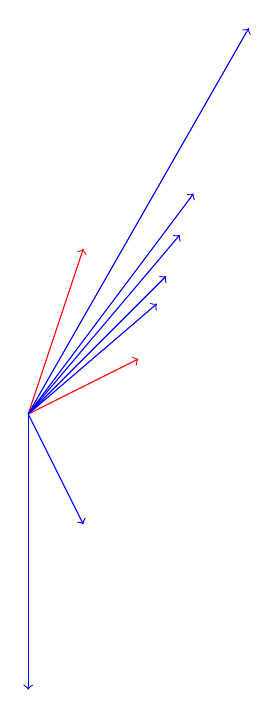
\begin{tikzpicture}[scale=.7]
	    % abscisa y ordenada
	    \tkzInit[xmax= 3,xmin=0,ymax=6,ymin=0]
	    \tiny\tkzLabelXY[opacity=0.6,step=1, orig=false]
	    % label x, f(x)
	    \tkzDrawX[opacity=0.6,label=x,right=0.3]
	    \tkzDrawY[opacity=0.6,label=f(x),below = -0.6]
	    \draw[red, ->](0,0)--(2,1);
	    \draw[red, ->](0,0)--(1,3);
	    \draw[blue, ->](0,0)--(7/3,2);
	    \draw[blue, ->](0,0)--(5/2,5/2);
	    \draw[blue, ->](0,0)--(11/4,13/4);
	    \draw[blue, ->](0,0)--(3,4);
	    \draw[blue, ->](0,0)--(4,7);
	    \draw[blue, ->](0,0)--(1,-2);
	    \draw[blue, ->](0,0)--(0,-5);
	\end{tikzpicture}
    \end{center}

%--------------------3.
\item resolver el ejercicio 2 si $C=tA+B$.\\\\
    Respuesta.-\; 
    \begin{center}
	\begin{tabular}{clcl}
	    Si&$t=\frac{1}{3}$&$\Longrightarrow$&$C=(\frac{5}{3},\frac{10}{3})$\\\\
	    Si & $t=\frac{1}{2}$ & $\Longrightarrow$ & $C=(2,\frac{7}{2})$ \\\\
	    Si & $t=1$ & $\Longrightarrow$ & $C=(\frac{5}{2},\frac{15}{4})$ \\\\
	    Si & $t=2$ & $\Longrightarrow$ & $C=(3,4)$ \\\\
	    Si & $t=-1$ & $\Longrightarrow$ & $C=(5,5)$ \\\\
	    Si & $t=-2$ & $\Longrightarrow$ & $C=(-1,2)$ \\\\
	    Si & $t=\frac{3}{4}$ & $\Longrightarrow$ & $C=(-3,1)$ \\\\
	\end{tabular}
    \end{center}
    \begin{center}
	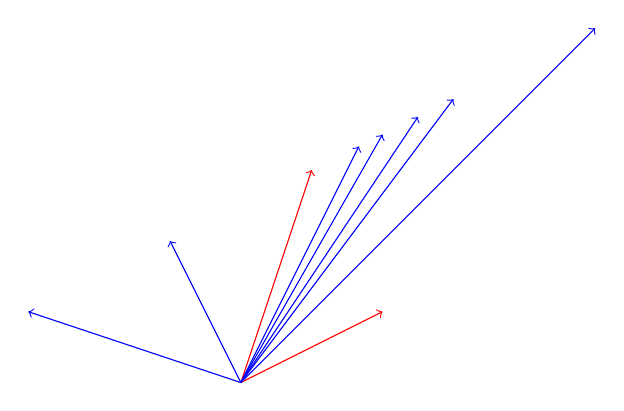
\begin{tikzpicture}[scale=.9]
	    % abscisa y ordenada
	    \tkzInit[xmax= 3,xmin=-3,ymax=3,ymin=0]
	    \tiny\tkzLabelXY[opacity=0.6,step=1, orig=false]
	    % label x, f(x)
	    \tkzDrawX[opacity=0.6,label=x,right=0.3]
	    \tkzDrawY[opacity=0.6,label=f(x),below = -0.6]
	    \draw[red, ->](0,0)--(2,1);
	    \draw[red, ->](0,0)--(1,3);
	    \draw[blue, ->](0,0)--(5/3,10/3);
	    \draw[blue, ->](0,0)--(2,7/2);
	    \draw[blue, ->](0,0)--(5/2,15/4);
	    \draw[blue, ->](0,0)--(3,4);
	    \draw[blue, ->](0,0)--(5,5);
	    \draw[blue, ->](0,0)--(-1,2);
	    \draw[blue, ->](0,0)--(-3,1);
	\end{tikzpicture}
    \end{center}

%--------------------4.
\item Sean $A=(2,1)$, $B=(1,3)$ y $C=xA+yB$, en donde $x$ e $y$ son escalares.
\begin{enumerate}[\bfseries a)]
    
    %----------a)
    \item Trazar el vector que une el origen a $C$ para cada uno de los siguientes pares de valores de $x$ e $y$: $x=y=\frac{1}{2}$; $x=\frac{1}{4},\;y = \frac{3}{4}$; $x=\frac{1}{3}, \; y=\frac{2}{3}$; $x=2,\; y=-1$; $x=3,\; y=-2$; $x=-\frac{1}{2},\; y=\frac{3}{2}$; $x=-1,\; y=2$.\\\\
	Respuesta.-\; 
	\begin{center}
	    \begin{tabular}{clcl}
		Si&$x=y=\frac{1}{2}$&$\Longrightarrow$&$C=\left(\frac{3}{2},2\right)$\\\\
		Si & $x=\frac{1}{4},\;y = \frac{3}{4}$ & $\Longrightarrow$ & $C=\left(\frac{5}{4},\frac{5}{2}\right)$ \\\\
		Si & $x=\frac{1}{3}, \; y=\frac{2}{3}$ & $\Longrightarrow$ & $C=\left(\frac{4}{3},\frac{7}{3}\right)$ \\\\
		Si & $x=2,\; y=-1$ & $\Longrightarrow$ & $C=(3,-1)$ \\\\
		Si & $x=3,\; y=-2$ & $\Longrightarrow$ & $C=(4,-3)$ \\\\
		Si & $x=-\frac{1}{2},\; y=\frac{3}{2}$ & $\Longrightarrow$ & $C=\left(\frac{1}{2},4\right)$ \\\\
		Si & $x=-1,\; y=2$ & $\Longrightarrow$ & $C=(0,5)$ \\\\
	    \end{tabular}
	\end{center}
	\begin{center}
	    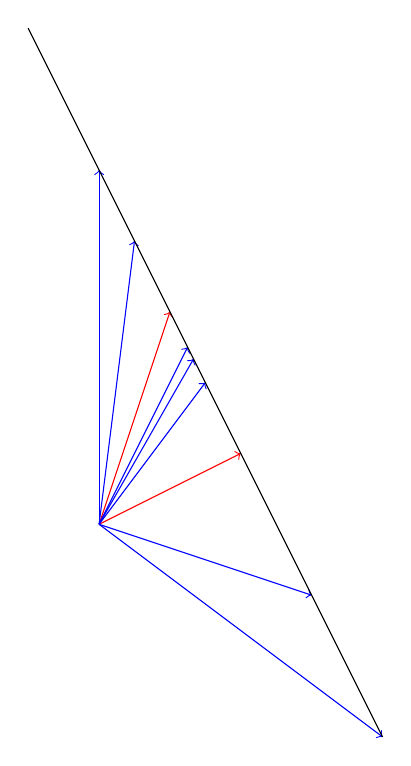
\begin{tikzpicture}[scale=.9]
		% abscisa y ordenada
		\tkzInit[xmax= 4,xmin=-3,ymax=4,ymin=-3]
		\tiny\tkzLabelXY[opacity=0.6,step=1, orig=false]
		% label x, f(x)
		\tkzDrawX[opacity=0.6,label=x,right=0.3]
		\tkzDrawY[opacity=0.6,label=f(x),below = -0.6]
		\draw[red, ->](0,0)--(2,1);
		\draw[red, ->](0,0)--(1,3);
		\draw[blue, ->](0,0)--(3/2,2);
		\draw[blue, ->](0,0)--(5/4,5/2);
		\draw[blue, ->](0,0)--(4/3,7/3);
		\draw[blue, ->](0,0)--(3,-1);
		\draw[blue, ->](0,0)--(4,-3);
		\draw[blue, ->](0,0)--(1/2,4);
		\draw[blue, ->](0,0)--(0,5);
		\draw[black](-1,7)--(4,-3);
	    \end{tikzpicture}
	\end{center}
    
    %----------b)
    \item ¿Qué conjunto es el de los puntos $C$ obtenidos cuando $x$ e $y$ toman todos los valores reales tales que $x+y=1$? (Hacer una conjetura y mostrar el lugar geométrico en la figura. No hacer la demostración).\\\\
	Respuesta.-\; Sea $x=3,\; y=-2$  y $x=-2,\; y=3$ podemos graficar el conjunto de los puntos $C$ tales que $x+y=1$.\\\\ 
    
    %----------c)
    \item Dar una idea del conjunto de todos los puntos $C$ obtenidos al variar independientemente $x$ e $y$ en los intervalos $0\leq x\leq 1, \; 0\leq y \leq 1,$ y hacer una representación de ese conjunto.\\\\
	Respuesta.-\; 
	\begin{center}
	    \begin{tikzpicture}[scale=.9]
		% abscisa y ordenada
		\tkzInit[xmax= 4,xmin=-3,ymax=4,ymin=-3]
		\tiny\tkzLabelXY[opacity=0.6,step=1, orig=false]
		% label x, f(x)
		\tkzDrawX[opacity=0.6,label=x,right=0.3]
		\tkzDrawY[opacity=0.6,label=f(x),below = -0.6]
		\draw[->](0,0)--(2,1);
		\draw[->](2,1)--(3,4);
		\draw[->](0,0)--(3,4);
	    \end{tikzpicture}
	\end{center}
    
    %----------d)
    \item ¿Qué conjunto es el de todos los puntos $C$ obtenidos si $x$ varía en el intervalo $0\leq x \leq 1$ e $y$ recorre todos los números reales?.\\\\
	Respuesta.-\; La banda horizontal obtenida sumando $xA$ a la línea $y = \frac{1}{3}x$ para cada uno $0 \leq x \leq 1$.\\\\

    %----------e)
    \item ¿Qué conjunto resulta si $x$ e $y$ recorren ambos todos los números reales?.\\\\
	Respuesta.-\; Todo $R^2$.\\\\

\end{enumerate}

%--------------------5.
\item Sean $A=(2,1)$ y $B=(1,3)$. Demostrar que todo vector $C=(c_1,c_2)$ de $V_2$ puede expresarse en la forma $C = xA+yB$. Expresar $x$ e $y$ en función de $c_1$ y $c_2$.\\\\
    Demostración.-\; Ya que $$C=xA+yB = (2x+y,x+3y)  = (c_1,c_2)$$
    se tiene $c_1 = 2x+y\;$ y $\;c_2 = x+3y$ de donde $$y=\dfrac{1}{5}(2c_2-c_1)$$  $$\;x=\dfrac{1}{5}(3c_1-c_2)$$
    Esto demuestra que cualquier vector en $\mathbb{R}^2$ se puede obtener como $xA+yB$ dado $C=(c_1,c_2)$ que calculamos.\\\\

%--------------------6.
\item Sea $A=(1,1,1)$, $B=(0,1,1)$ y $C=(1,1,0)$ tres vectores de $V_3$ y $D=xA+yB+zC$, donde $x$, $y$ $z$ son escalares.
\begin{enumerate}[\bfseries a)]

    %----------a)
    \item Determinar los componentes de $D$.\\\\
	Respuesta.-\; Tenemos que $D=x(1,1,1)+y(0,1,1)+z(1,1,0)$ de donde $D=(x,x,x)+(0,y,y)+(z,z,0)$
	así, $$D=(x+z,x+y+z,x+y)$$\\

    %----------b)
    \item Si $D=0$ demostrar que $x=y=z=0$.\\\\
	Demostración.-\; Sea $D=0=(0,0,0)$ entonces 
	\begin{center}
	    \begin{tabular}{rcl}
		$x+z=0$&$\Longrightarrow$&$x=-z$\\	
		$x+y+z=0$&$\Longrightarrow$&$y=0$\\
		$x+y=0$&$\Longrightarrow$&$x=-y$\\
	    \end{tabular}
	\end{center}
	de donde concluimos que $x=y=z=0$.\\\\

    %----------c)
    \item Hallar $x, y, z$ tales que $D=(1,2,3)$.\\\\
	Respuesta.-\; 
	\begin{center}
	    \begin{tabular}{rcll}
		$x+z=1$&$\Longrightarrow$&$z=1-x$&$\Longrightarrow z=-1$\\
		$x+y+z=2$&$\Longrightarrow$&$x+y+1-x=2$&$\Longrightarrow y=1$\\
		$x+y=3$&$\Longrightarrow$&$x+1=3$&$\Longrightarrow x=2$\\\\
	    \end{tabular}
	\end{center}

\end{enumerate}

%--------------------7.
\item Sean $A=(1,1,1)$, $B=(0,1,1)$ y $C=(2,1,1)$ tres vectores de $V_3$ y $D=xA+yB+zC$, en donde $x,y,z$ son escalares.
\begin{enumerate}[\bfseries a)]

    %----------a)
    \item Determinar los componentes de $D$.\\\\
	Respuesta.-\; Sea $D=x(1,1,1)+y(0,1,1)+z(2,1,1)$ entonces $D=(x+2z,x+y+z,x+y+z)$.\\\\


    %----------b)
    \item Hallar $x,y,z$ no todos nulos, tales que $D=0$.\\\\
	Respuesta.-\; Sea $x=2$, $y=-1$ y $z=-1$, entonces $$D=(x+2z,x+y+z,x+y+z)=(2-2,2-1-1,2-1-1)=(0,0,0)=O$$ \\

    %----------c)
    \item Demostrar que ninguna elección de $x,y,z$ hace $D=(1,2,3)$.\\\\
	Demostración.-\; Sea 
	\begin{center}
	    \begin{tabular}{rcll}
		$x+2z=1$&$\Longrightarrow$&$x=1-2z$&\\
		$x+y+z=2$&$\Longrightarrow$&$1-2z+y+z=2$&$\Longrightarrow y=z+1$\\
		$x+y+z=3$&$\Longrightarrow$&$1-2z+z+1+z=3$&$\Longrightarrow 2=3$\\
	    \end{tabular}
	\end{center}
	de donde encontramos un absurdo al declarar que $2=3$, por lo tanto no existe ninguna elección que satisfaga a $D=(1,2,3)$.\\\\

\end{enumerate}

%--------------------8.
\item Sean $A=(1,1,1,0)$, $B=(0,1,1,1)$, $C=(1,1,0,0)$ tres vectores de $V_4$ y $D=xA+yB+zC$ siendo $x,y,z$ escalares.
\begin{enumerate}[\bfseries a)]

    %----------a)
    \item Determinar los componentes de $D$.\\\\
	Respuesta.-\; Se tiene $D=x(1,1,1,0)+y(0,1,1,1)+z(1,1,0,0)$ entonces $D=(x+z,x+y+z,x+y,y)$\\\\

    %----------b)
    \item Si $D=0$, Demostrar que $x=y=z=0$\\\\
	Respuesta.-\; 
	\begin{center}
	\begin{tabular}{rcl}
	    $x+z=0$&&\\
	    $x+y+z=0$&$\Longrightarrow$&$z=0$\\
	    $x+y=0$&$\Longrightarrow$&$x=0$\\
	    $y=0$&&\\
	\end{tabular}
	\end{center}
	Por lo tanto $x=y=z=0$.\\\\

    %----------c)
    \item Hallar $x,y,z$ tales que $D=(1,5,3,4)$.\\\\
	Respuesta.-\;
	\begin{center}
	\begin{tabular}{rcl}
	 $x+z=1$&&\\
	 $x+y+z=5$&$\Longrightarrow$&$z=2$\\
	 $x+y=3$&$\Longrightarrow$&$x=-1$\\
	 $y=4$&&\\
	\end{tabular}
	\end{center}
	Por lo tanto $x=-1$, $y=4$ y $z=2$.\\\\

    %----------d)
    \item Demostrar que ninguna elección de $x,y,z$ hace $D=(1,2,3,4)$.\\\\
	Demostración.-\; La demostración es similar al problema 7c.\\\\

\end{enumerate}

%--------------------9.
\item En $V_n$ demostrar que dos vectores paralelos a un mismo vector son paralelos entre sí.\\\\
    Demostración.-\; Por definición de vectores paralelos se tiene $c_1A=C$ y $c_2B=C$ de donde $c_1A=c_2B$, en vista de que $c_1\cdot c_2 \neq 0$ entonces $B=c_1c_2^{-1} A$, por lo tanto concluimos que $A$ y $B$ son paralelos entre sí.\\\\ 

%--------------------10.
\item Dados cuatro vectores no nulos $A,B,C,D$ de $V_n$ tales que $C=A+B$ y $A$ paralelo a $D$. Demostrar que $C$ es paralelo a $D$ si y sólo si $B$ es paralelo a $D$.\\\\
    Demostración.\; 

%--------------------11.
\item 
\begin{enumerate}[\bfseries a)]
    
    %----------a)
    \item Demostrar, para los vectores $V_n$ las propiedades de la adición y de la multiplicación oor escalares dadas en el teorema 12.1\\\\
	Demostración.-\; 

    %----------b)
    \item Mediante vectores geométricos en el plano, representar el significado geométrico de las dos leyes distributivas $(c+d)A=cA+dA$ y $c(A+B) = cA+cB$.\\\\
	Respuesta.-\;

\end{enumerate}

%--------------------12.
\item Si un cuadrilátero $OABC$ de $V_2$ es un paralelogramo que tiene $A$ y $C$ como vértices opuestos, demostrar que $A+\frac{1}{2}(C-A) =\frac{1}{2}B$. ¿Qué teorema relativo a los paralelogramos puede deducirse de esta igualdad?.\\\\
    Demostración.-\; 

\end{enumerate}
